% annexes, numérotées en lettres (A, B, ...)
\appendix
% page en paysage pour que le chronogramme du chenillard soit lisible sur une seule page
\begin{landscape}
	\enteteEtPiedPaysage
	\section{Annexes}
	\subsection{Chronogramme de la simulation du chenillard}
	\label{annexe:simu_p3}

	Chronogramme complet de la simulation du chenillard (partie 3), commenté à la section Simulation. Il est découpé en deux parties pour garder une bonne lisibilité.

	\begin{chronogramme}
		\centering
		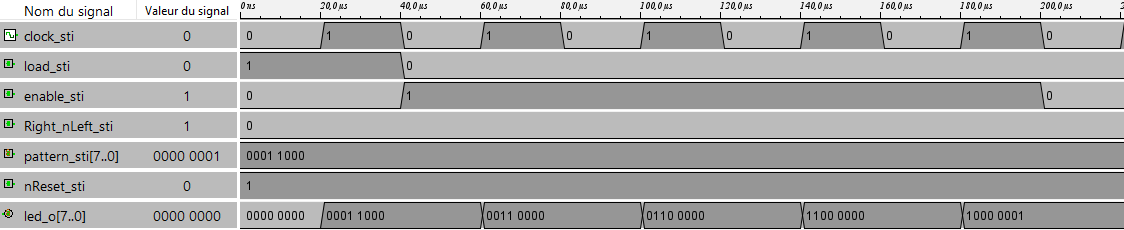
\includegraphics[width=0.85\linewidth]{./images/simulation-partie3-a.png}

		\vspace{0.3cm}
		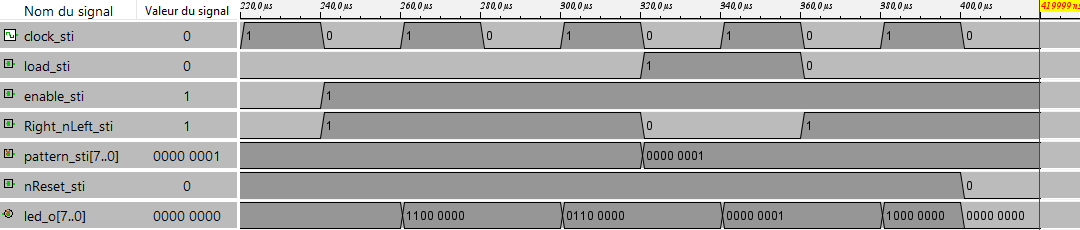
\includegraphics[width=0.85\linewidth]{./images/simulation-partie3-b.png}
		\caption{Partie 3, simulation Logisim, chenillard}
		\label{fig:simu_p3}
	\end{chronogramme}
\end{landscape}

\subsection{Fichier de projet Logisim}
\label{annexe:circ}

Le fichier \texttt{srg8\_ld\_sh.circ} est le fichier de projet Logisim de ce laboratoire. Il est fourni avec ce rapport dans l'archive \texttt{rendu.zip}.
